%%\newpage
\section{Mono-Bass-Addier-Schaltung und Mono-Bass-Weiche}\label{kap:5.1}
\subsection{Allgemeines}\label{kap:5.1.1}
Das empfangene Audio-Signal muss für das Lautsprecher-System aufgetrennt werden. In Hoch, Mitte und Tief Audiofrequenz. Für den \enquote{Mono-Bass} werden nur die tiefen Frequenzen des Signals gebraucht. Da, wie der Name schon sagt, es sich um einen \enquote{Mono-Bass} handelt, muss das Stereo-Audio-Signal vorher noch mittels OPV-Addierschaltung addiert werden um ein Mono-Audio-Signal zu erhalten.

\subsection{Zielsetzung}\label{kap:5.1.2}
Es soll ein Print angefertigt werden, welcher über eine OPV-Addierschaltung verfügt und des weiteren das eintreffende Audio-Signal über ein Filter passend für den \enquote{Mono-Bass} filtert.
Diese Schaltung für das Tiefpass-Filter muss variabel designet werden. Das Tiefpass-Filter muss unabhängig vom Printdesign, nur durch Ändern von Bauteilwerten, andere Grenzfrequenzen liefern können.

\subsection{Auswahl des Tiefpass-Filters}\label{kap:5.1.3}
Es wurde nach einem möglichst steilen, im Durchlassbereich linearen und einfachen Tiefpass-Filter gesucht. Man hat sich nach Überlegen für ein \enquote{Aktives-Tiefpass-Filter 2.Ordnung} entschieden, dabei wurde die \enquote{Butterworth-Schaltung} bevorzugt. Wegen seiner hohen Linearität im Durchlassbreich und einer Dämpfung von $\frac{-20dB}{Dek.}$ . Dies bedeutet, dass eine Frequenz die 10mal größer ist als die Grenzfrequenz einen um $\frac{1}{10}$ kleineren Pegel aufweist, als die Grenzfrequenz.\\
Zur Regelung wird an den Eingängen (Rechts, Links) und am Ausgang der Schaltung jeweils ein Potentiometer in der Größenordnung von 1kOhm verbaut. Diese dienen zur Anpassung der Amplitude des ein- und ausgehenden Signals, um mögliche Übersteuerungen zu vermeiden.

\subsection{Butterworth-Filter 2. Ordnung}\label{kap:5.1.4}
Die Grundschaltung eines Butterworth-Tiefpass-Filter 2. Ordnung ist auch bei verschieden Grenzfrequenzen gleich. Es besteht hauptsächlich aus einem OPV, drei Widerständen und zwei Kondensatoren. Deren Anordnung ist ausschlaggebend für das Tiefpass-Filter (Abb. \ref{fig:abb5.1.4.1}).\\ 
Bedingt durch das Beschalten des OPVs wird das Ausgangssignal invertiert, was hier keine gröberen Folgen mit sich bringt.\\ 
Am Plus-Eingang des OPVs wird entweder Masse bei symmetrischer Spannungsversorgung, oder $\frac{Vcc}{2}$ bei asymmetrischer Spannungsversorgung angelegt.
\begin{figure} [h]
	\centering
	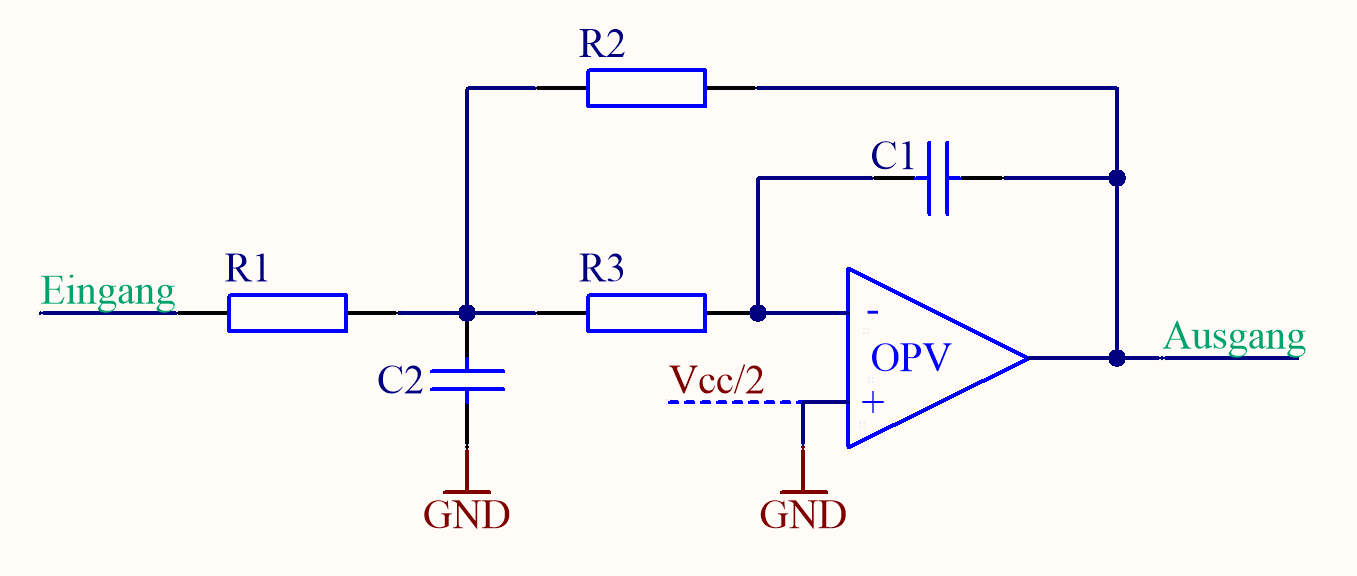
\includegraphics[width=1\textwidth]{img/Print3/TPFilterButterworth2Ordnung.PNG}
	\caption{Butterworth-Filter 2. Ordnung}
	\label {fig:abb5.1.4.1}
\end{figure}\\

\subsection{Schaltung}\label{kap:5.1.5}
Passend dem Signalverlauf sitzt am Beginn der Schaltung (Abb. \ref{fig:abb5.1.5.1}) die erste Regelung über Potentiometer. Anschließend kommt man zu der Addier-Schaltung (Abb. \ref{fig:abb5.1.5.2}) welche das Stereo-Signal in ein Mono-Signal wandelt und dadurch Stereo-Effekte wie zB. Balance am \enquote{Mono-Bass} entfernt.\\
Wichtig ist bereits hier die Versorgung der Schaltung. Bedingt durch eine asymmetrische Spannungsversorgung (0...12V) muss am OPV ein Arbeitspunkt eingestellt werden. Dabei handelt es sich um ein absichtliches Anheben des Signals in Y-Richtung bei einem Spannungs-Zeit-Verlauf, sodass die untere Halbwelle des Signals nicht verloren geht. Dafür muss am Plus-Eingang des OPVs der Addier-Grundschaltung und der Butterworth-Filter-Schaltung die halbe Versorgungsspannung angelegt werden, um das beste Ergebnis zu erzielen. Dafür wird an den beiden Plus-Eingängen der OPVs über eine Spannungsteiler-Schaltung aus zwei Widerständen das benötigte $\frac{Vcc}{2}$ angelegt.\\
Um Störungen im OPV zu vermeiden wird sehr nahe an diesem ein 10µF ELKO in der Versorgungsspannungsleitung vorgesehen.\\
Nach Addieren des Stereo-Signals zu einem Mono-Signal kommt dieses zum Aktiven-Tiefpass-Filter(Abb. \ref{fig:abb5.1.5.3}). Bevor das gefilterte Signal weiter zum Verstärker geht wird nochmals die Möglichkeit geboten um die Amplitude des Signals anzupassen.
\begin{figure} [h]
	\centering
	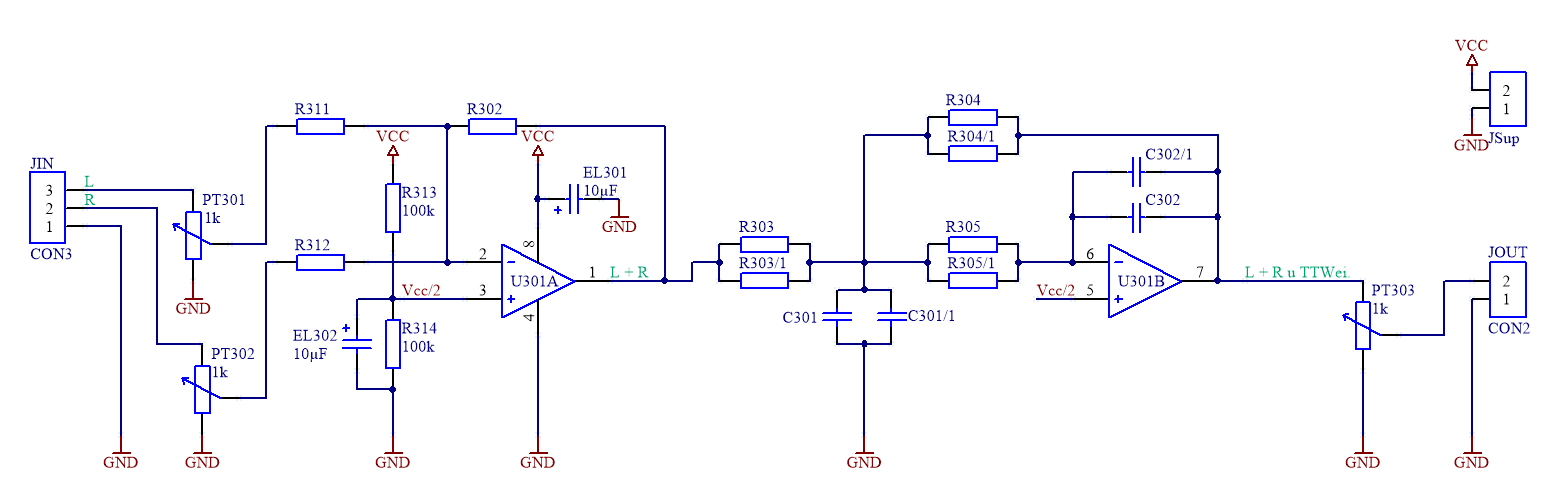
\includegraphics[width=0.8\textwidth]{img/Print3/3mTTWeicheruAddiererDiplSchematic.PNG}
	\caption{Schematic Mono-Bass-Addier-Schaltung und Mono-Bass-Weiche}
	\label {fig:abb5.1.5.1}
\end{figure}
\begin{figure} [h]
	\centering
%	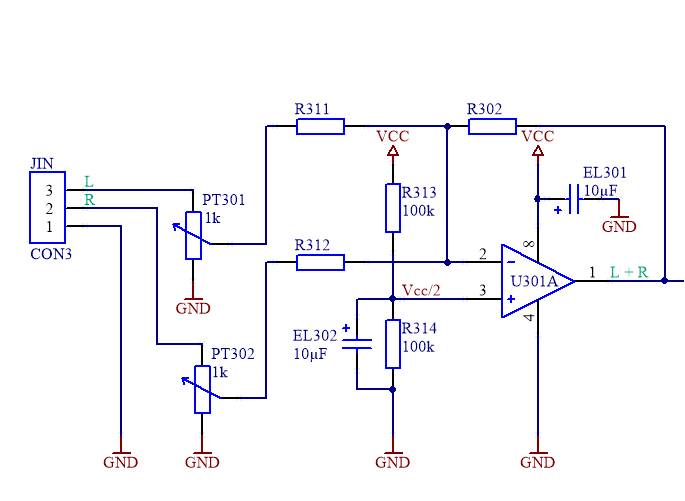
\includegraphics[width=0.8\textwidth]{img/Print3/3mTTWeicheruAddiererDiplSchematicTeil1.png}
	\caption{Schematic Mono-Bass-Addier-Schaltung}
	\label {fig:abb5.1.5.2}
\end{figure}
\begin{figure} [h]
	\centering
%	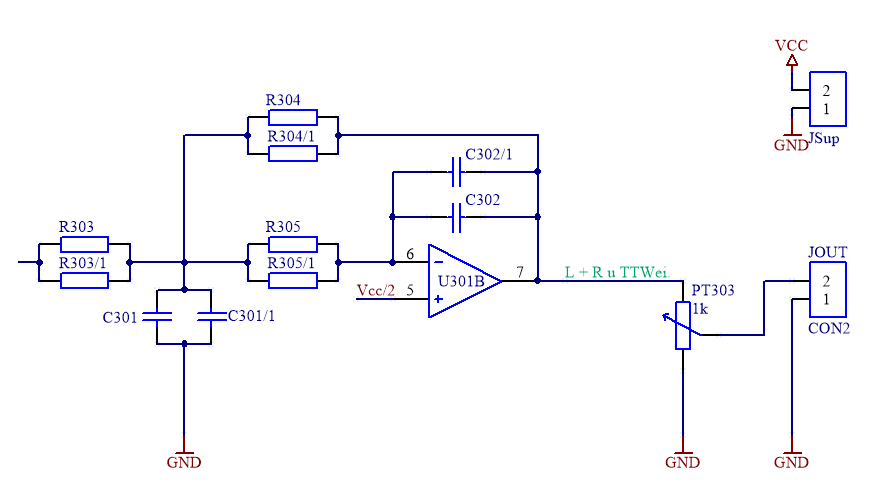
\includegraphics[width=0.8\textwidth]{img/Print3/3mTTWeicheruAddiererDiplSchematicTeil2.png}
	\caption{Schematic Mono-Bass-Weiche}
	\label {fig:abb5.1.5.3}
\end{figure}

\subsection{PCB}\label{kap:5.1.6}
An einer der vier Seiten der Leiterplatte(Abb. \ref{fig:abb5.1.6.1}) wurden alle wesentlichen Ein- und Ausgänge platziert. Eine dreipolige Eingangsstiftleiste für Rechts, Links und Masse. Eine zweipolige Ausgangsstiftleiste für Signal und Masse. Des weiteren darf die Spannungsversorgung nicht fehlen. Wegen größeren Spannungen wurden massivere Stecker verwendet. In diesem Fall handelt es sich um Pol-Klemmen. Zum testen wurde ein zusätzlicher Masse-Printstift angebracht um bei Messungen mit einem Oszilloskop einem besseren Massebezugpunkt zu haben.\\
Die Bauteile wurden nach Möglichkeit gestaffelt, beziehungsweise gruppiert auf der Leiterplatte platziert um den Platzbedarf zu minimieren.\\
Es wurde grundsätzlich auf jeden Print versucht eine geeignete Beschriftung vor zu sehen um Außenstehenden die Handhabung mit dem Print ebenfalls zu ermöglichen. Masse wurde selten Beschriftet, da eine Massefläche verwendet wurde und daher die Massepins sehr gut ersichtlich sind.
\begin{figure} [h]
	\centering
	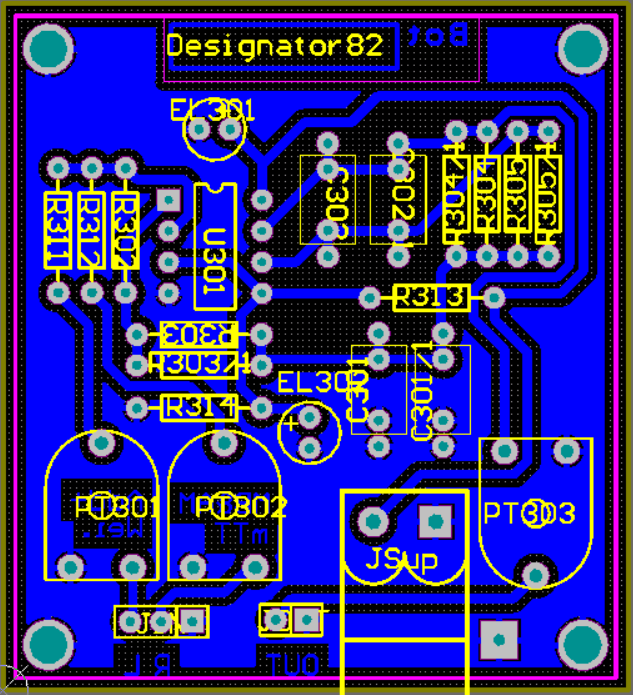
\includegraphics[width=0.8\textwidth]{img/Print3/3mTTWeicheruAddierer-PCB.PNG}
	\caption{PCB}
	\label {fig:abb5.1.6.1}
\end{figure}




\begin{comment}
%% Altium und Einstellungserklärung + Wichtige Layout-Faktoren
%Beim designen des Leiterplattenlayouts wurden die allgemeinen Altium-Einstellungen vorgenommen und auf die zu berücksichtigenden Layoutpunkte geachtet.
Beim \enquote{Layouten} der Schaltung mussten einige wichtige Faktoren berücksichtigt werden.\\
Wie da wären:\\
\begin{itemize}
	\item EMV-Technische-Faktoren, wie kurze Leiterbahnen
	\item Ausnützen der Printfläche
	\item Mehrfach-Footprints ermöglichen für verschiedene Bauteile
	\item Mechanische Aufhängebohrungen vorsehen
	\item Massefläche bei Möglichkeit vorsehen
\end{itemize}
Leiterplattenspezifische Einstellungen wurden aus den Kriterien der schuleigenen Leiterplattenfertigung übernommen. Zu diesen Einstellungen zählen:\\
\begin{itemize}
	\item Leiterbahnbreite
	\item Leiterbahnabstände untereinander
	\item Restring bei Bohrungen
	\item 
\end{itemize}
\end{comment}







